\documentclass[tikz,border=12pt]{standalone}
\usepackage[T1]{fontenc}
\usepackage{mathpazo}
\usepackage{amsmath,amssymb}
\usetikzlibrary{arrows.meta, positioning, calc, fit, decorations.pathreplacing}
\usepackage{pgfplots}
\pgfplotsset{compat=1.18}

\definecolor{stblue}{HTML}{7B97AD}
\definecolor{rwgold}{HTML}{B8995E}
\definecolor{sage}{HTML}{7A9A7E}
\definecolor{dkbrown}{HTML}{3D3530}
\definecolor{wmgray}{HTML}{7B7067}
\definecolor{cream}{HTML}{F9F6F0}
\definecolor{border}{HTML}{D4C9B8}
\definecolor{terracotta}{HTML}{C47A6A}
\definecolor{lavender}{HTML}{907EA0}

\begin{document}
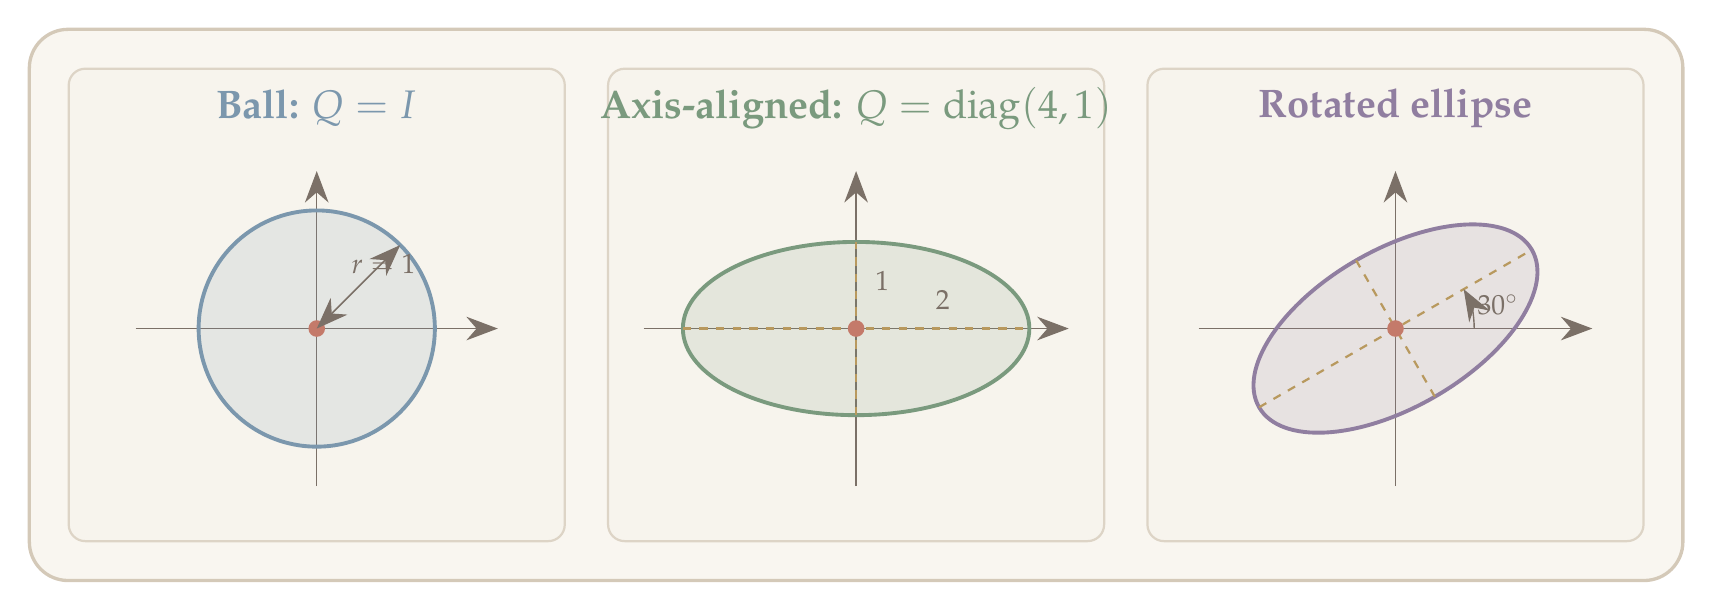
\begin{tikzpicture}[>={Stealth[length=4mm, width=3mm]}, line width=1.5pt]

% Background
\fill[cream, rounded corners=14pt] (-0.5,-3.2) rectangle (20.5,3.8);
\draw[border, line width=1.2pt, rounded corners=14pt] (-0.5,-3.2) rectangle (20.5,3.8);

%%% Panel 1: Ball Q = I %%%
\fill[cream!95!border, rounded corners=6pt] (0.0,-2.7) rectangle (6.3,3.3);
\draw[border!80, line width=0.8pt, rounded corners=6pt] (0.0,-2.7) rectangle (6.3,3.3);
\node[text=stblue, font=\Large\bfseries] at (3.15,2.8) {Ball: $Q = I$};

\begin{scope}[shift={(3.15,0.0)}]
  % Axes
  \draw[wmgray, line width=0.5pt, ->] (-2.3,0) -- (2.3,0);
  \draw[wmgray, line width=0.5pt, ->] (0,-2.0) -- (0,2.0);
  % Circle
  \fill[stblue, opacity=0.15] (0,0) circle (1.5cm);
  \draw[stblue, line width=1.4pt] (0,0) circle (1.5cm);
  % Center dot
  \fill[terracotta] (0,0) circle (3pt);
  % Radius annotation
  \draw[wmgray, line width=0.6pt, <->] (0,0) -- (1.06,1.06);
  \node[text=wmgray, font=\normalsize, anchor=south west] at (0.3,0.55) {$r=1$};
\end{scope}

%%% Panel 2: Axis-aligned Q = diag(4,1) %%%
\fill[cream!95!border, rounded corners=6pt] (6.85,-2.7) rectangle (13.15,3.3);
\draw[border!80, line width=0.8pt, rounded corners=6pt] (6.85,-2.7) rectangle (13.15,3.3);
\node[text=sage, font=\Large\bfseries] at (10.0,2.8) {Axis-aligned: $Q = \mathrm{diag}(4,1)$};

\begin{scope}[shift={(10.0,0.0)}]
  % Axes
  \draw[wmgray, line width=0.5pt, ->] (-2.7,0) -- (2.7,0);
  \draw[wmgray, line width=0.5pt, ->] (0,-2.0) -- (0,2.0);
  % Ellipse: semi-axes 2 and 1
  \fill[sage, opacity=0.15] (0,0) ellipse (2.2cm and 1.1cm);
  \draw[sage, line width=1.4pt] (0,0) ellipse (2.2cm and 1.1cm);
  % Dashed principal axes
  \draw[rwgold, line width=0.8pt, dashed] (-2.2,0) -- (2.2,0);
  \draw[rwgold, line width=0.8pt, dashed] (0,-1.1) -- (0,1.1);
  % Center dot
  \fill[terracotta] (0,0) circle (3pt);
  % Semi-axis annotations
  \node[text=wmgray, font=\normalsize, anchor=south] at (1.1,0.1) {$2$};
  \node[text=wmgray, font=\normalsize, anchor=west] at (0.1,0.6) {$1$};
\end{scope}

%%% Panel 3: Rotated ellipse %%%
\fill[cream!95!border, rounded corners=6pt] (13.7,-2.7) rectangle (20.0,3.3);
\draw[border!80, line width=0.8pt, rounded corners=6pt] (13.7,-2.7) rectangle (20.0,3.3);
\node[text=lavender, font=\Large\bfseries] at (16.85,2.8) {Rotated ellipse};

\begin{scope}[shift={(16.85,0.0)}]
  % Axes
  \draw[wmgray, line width=0.5pt, ->] (-2.5,0) -- (2.5,0);
  \draw[wmgray, line width=0.5pt, ->] (0,-2.0) -- (0,2.0);
  % Rotated ellipse: 30 degrees, semi-axes 2 and 1
  \fill[lavender, opacity=0.15, rotate=30] (0,0) ellipse (2.0cm and 1.0cm);
  \draw[lavender, line width=1.4pt, rotate=30] (0,0) ellipse (2.0cm and 1.0cm);
  % Dashed principal axes (rotated 30 degrees)
  \draw[rwgold, line width=0.8pt, dashed] ({-2.0*cos(30)},{-2.0*sin(30)}) -- ({2.0*cos(30)},{2.0*sin(30)});
  \draw[rwgold, line width=0.8pt, dashed] ({-1.0*cos(120)},{-1.0*sin(120)}) -- ({1.0*cos(120)},{1.0*sin(120)});
  % Center dot
  \fill[terracotta] (0,0) circle (3pt);
  % Angle arc
  \draw[wmgray, line width=0.5pt, ->] (1.0,0) arc[start angle=0, end angle=30, radius=1.0cm];
  \node[text=wmgray, font=\normalsize] at (1.3,0.3) {$30^\circ$};
\end{scope}

\end{tikzpicture}
\end{document}
